\documentclass[11pt]{article}
\usepackage{geometry}                % See geometry.pdf to learn the layout options. There are lots.
\geometry{letterpaper}                   % ... or a4paper or a5paper or ... 
%\geometry{landscape}                % Activate for for rotated page geometry
%\usepackage[parfill]{parskip}    % Activate to begin paragraphs with an empty line rather than an indent
\usepackage{graphicx}
\usepackage{amssymb}
\usepackage{epstopdf}
\usepackage{amsmath}
\DeclareGraphicsRule{.tif}{png}{.png}{`convert #1 `dirname #1`/`basename #1 .tif`.png}


\title{Mathematical representation of the drought decision model - Shiny Version}
\author{Trisha Shrum}
%\date{}                                           % Activate to display a given date or no date

\begin{document}
\maketitle
%\section{}
%\subsection{}

\section{Model}
In this model, ranchers maintain a herd of cows to produce calves for sale at market. The variable inputs to the production of calves are cows and forage. Forage availability is determined by rainfall, which is determined exogenously by drawing from historical rain gauge records, and hay, which may be purchased on an annual basis. The number of cows in a herd can be increased or decreased by selling cows and calves. 

Year is indexed with $t$ and month is indexed with $i$. The goal of the player is to maximize the following objective function:

\begin{equation}
\label{objFunction}
\max_{a_t, x_t, y_t} \sum_{t=1}^T \pi_t(1+r)^{-t}
\end{equation}

subject to constraints on herd growth and forage potential as well as constraints on a number of key variables described in the sections that follow.

\subsection{Stock Variables}
Two variables, herd size and forage potential are stock variables that depend on their values in previous years and other key factors. 

\subsubsection{Herd Size}
Herd size, $\theta_t$, is a stock variable that grows or shrinks according to the following equation:
\begin{equation}
\label{herdSize}
\theta_t = \theta_{t-1} (1- d_{t-1}) (1 - y_{t-1}) + \theta_{t-2} \omega_{t-2} (1 - x_{t-2})
\end{equation} 
where $d_{t}$ is the death rate of cows, $y_{t}$ is the percentage of cows sold in year $t$, $\omega_t$ is the percentage of cows who successfully birth and wean a calf in year $t$ (referred to as weaning percentage), and $x_t$ is the percentage of calves sold in year $t$. 

In the simulation, we set the death rate of cows, $d_t$, to a constant value of 4\% per year. In future work, the death rate could more realistically depend on forage availability, extreme heat exposure, and age. 

The percentage of calf and cow sales, $x_t$ and $y_t$, are choice variables. In the simulation, the player chooses how many cows and calves to sell at the end of each growing season. The lower bound on calf sales is 50\% due to the fact that male calves do not have economic value in a cow-calf operation. The lower bound on cow sales is 0\%. We make the simplifying assumption of no relationship between culling cows and average weaning percentage. In reality, a cow-calf operation sells cows that do not produce calves in order to keep the herd at optimal calve production. If they do not sell calves, the weaning percentage would begin to fall. We justify this simplification by assuming a young herd that is not yet experiencing declining fertility due to age and by assuming that all cows have an equal likelihood of producing a calf in a given year. 

The weaning percentage, $\omega_t$, depends on the health of the herd in year $t$ and year $t-1$, which is assumed to be fully based on total available forage per cow, $\lambda_t$ and $\lambda_{t-1}$. In the simulation, the weaning percentage maximum is 88\%, represented by $\tilde{\omega}$. Weaning percentage in year $t$, $\omega_t$, is given by:\\

\begin{equation}
\label{weaningPercentage}
\omega_t =
\begin{cases}
\tilde{\omega}  &\text{if } \lambda_{t}, \lambda_{t-1} \ge 1  \\
\tilde{\omega} * \lambda_{t}^{(1/4)} &\text{if } \lambda_{t} < 1 \land \lambda_{t-1} \ge 1 \\
\tilde{\omega} * \lambda_{t - 1} &\text{if } \lambda_{t} \ge 1 \land \lambda_{t-1} < 1 \\
\tilde{\omega} * \lambda_{t}^{(1/4)} * \lambda_{t-1} &\text{if } \lambda_{t}, \lambda_{t-1} < 1 \\
\end{cases}
\end{equation}

Forage availability, $\lambda_t$, is further described in section \ref{forage}.

\subsubsection{Forage Potential}
Forage potential is a vector that translates monthly rainfall into annual forage production. It is a stock variable that changes according to the following equation:
\begin{align}
\label{foragePotential}
\vec{\alpha}_t &= \vec{\alpha}_{t-1} \left(1 - \frac{G_{t-1}}{x}\right), \\
&\text{ where } \tilde{\alpha} \equiv \sum_{i=1}^{12} \alpha_{i}  \le 1 \label{maxforagePotential}
\end{align}

Forage potential increases or decreases based on the grazing pressure, $G_t$, on the land. If $G_t < 0$, then forage potential increases (subject to a maximum, $\tilde{\alpha}$, defined in eq. \ref{maxforagePotential}). This maximum is the starting point of the model and is determined by the MLRA plant growth curves.  If $G_t > 0$, then forage potential decreases (subject to a minimum of 0). 

For each monthly value in the vector $\alpha_{t}$, the previous years' forage value is multiplied by a percentage that is determined by the grazing pressure and a scaling factor, $x$. The parameter $x$ allows for the impact of grazing pressure on forage potential to vary for different rangeland ecosystems. In the simulation where we model grazing at the Central Plains Experimental Range (CPER), $x=1$. This parameterization follows the advice recommended by a team of ranching experts at the University of Wyoming who study the CPER.\footnote{The expert team consulted included Justin Derner, Dannele Peck, John Ritten, and John Hewlett.} They suggested that forage potential would decrease by 1-2\% per year when grazing pressure is relatively high. %CHECK ON THIS. WHAT IS THE RELATIONSHIP BETWEEN GRAZING PRESSURE AND FORAGE POTENTIAL? WHAT DO WE SEE UNDER A REASONABLE RANGE OF CIRCUMSTANCES?

Grazing pressure, $G_t$, depends on forage production, $F_t$, herd size, $\theta_t$, and the level of investment in drought adaptation, $a_t$:
\begin{equation}
G_t = 1 - (F_t + a_t)
\end{equation}

At a sustainable equilibrium, $G_t = 0$. We define this equilibrium as follows: when forage production per pair plus drought adaptation measures are equal to 1, then there is zero grazing pressure. As forage production per pair plus drought adaptation measures fall below 1, then there is positive grazing pressure leading to a degradation of forage potential. As forage production per pair plus drought adaptation measures rise above 1, then there is negative grazing pressure leading to a recovery of forage potential if it is not already at full health, $\tilde{\alpha}$.  

\subsubsection{Forage Availability}
\label{forage}
Forage availability per cow-calf pair is equal to the sum of forage production, $F_t$, and drought adaptation, $a_t$:
\begin{equation}
\lambda_t = F_t + a_t
\end{equation}

Forage production per pair, $F_t$, is the dot product of forage potential, $\alpha_t$, and the monthly rainfall, $\rho_t$, divided by the ratio of acres per cow and carrying capacity. $\alpha_t$ and $\rho_t$ are vectors with a length of twelve representing each month of the year. 
\begin{equation}
F_t = \frac{\alpha_t \cdot \rho_t}{\%K}
\end{equation}

In an average rainfall year with undegraded forage potential, if the herd size is equal to the carrying capacity, then $F_t = 1$. As rainfall or forage potential increases (decreases), $F_t$ increases (decreases). As herd size increases (decreases), $F_t$ decreases (increases). 

Carrying capacity, $\%K$, is defined as follows:
\begin{equation}
\%K = \frac{\frac{l}{\theta_t}}{K}
\end{equation}
where $l$ is the number of acres grazed, $\theta_t$ is the size of the herd (head of cows, not including calves or yearlings), and $K$ is defined as the sustainable carrying capacity of the ranch in an average year (acres/cow).

When the herd is at its carrying capacity ($l/\theta_t = K)$, $\%K$ = 1. When the carrying capacity is exceeded, $\%K > 1$, leading to a reduction of forage per pair. In other words, at any given level of forage potential and rainfall, the forage per pair is smaller when the herd increases. Likewise, when $l / \theta_t < K$, the forage per pair increases (holding forage and rainfall constant). 

Perfect adaptation, $\hat{a}_t$, is defined as the gap between full forage production per pair ($F_t = 1$) and actual forage production per pair. It is a unitless measure that is best interpreted as a percentage.
\begin{equation}
\hat{a}_t \equiv 1 - F_t
\end{equation}

Actual adaptation, $a_t$, is defined as the portion of the gap between full forage production per pair and actual forage production per pair that is filled with drought adaptation measures, such as the purchase of additional feed. We define this as the ratio of expenditures on adaptation and cost of perfect adaptation scaled by the perfect adaptation, $\tilde{a}_t$. We assume that the costs of adaptation are linear. 
\begin{equation}
a_t \equiv \frac{\text{Expenditures on adaptation}}{C(\tilde{a}_t)} \tilde{a}_t
\end{equation}


Additional parameter constraints (bring into the discussion of the model):
\begin{equation}
w_t \in [0,\tilde{w}]
\end{equation}

\begin{equation}
\omega_t \in [0,\tilde{\omega}]
\end{equation}

\begin{equation}
x_t \in [0.5,1]
\end{equation}

\begin{equation}
a_t, d_t, y_t \in [0,1]
\end{equation}

\begin{equation}
F_t, p_t, \rho_t, l, \theta_t \ge 0 
\end{equation}

\subsection{Overview of variables:}
\begin{itemize}

\item Choice Variables
\begin{description}
\item[$a_t$]: Adaptation (\%)
\item[$x_t$]: Percentage of calves sold (\%)
\item[$y_t$]: Percentage of cows sold (\%)
\end{description}

\item Stock Variables
\begin{description}
\item[$\theta_t$]: Herd size (cows, not including calves and yearlings). Herd size in year $t$ is a function of herd size in the previous year, $\theta_{t-1}$, percentage of cows culled in the previous year, $z_{t-1}$, death rate of cows in the previous year, $d_{t-1}$, herd size two years prior, $\theta_{t-2}$, weaning percentage two years prior, $y_{t-2}$, and percentage of calves sold two years prior, $m_{t-2}$. This implicitly assumes that all yearlings survive to become mature cows.
\item[$\alpha_t$]: Forage potential (\%) (stock variable)
\end{description}

\item Response variables
\begin{description}
\item[$\pi_t$]: Profit in year t (\$)
\item[$G_t$]: Grazing pressure, $G_t$, depends on the forage production, the herd size, and the level of investment in adaptation. 
At a sustainable equilibrium, $G_t = 0$. 
\item[$w_t$]: Average weaning weight (pounds) subject to a maximum weight $\tilde{w}$ (default value of $\tilde{w}= 600$ pounds).
\item[$\omega_t$]: Weaning percentage (\%) subject to a maximum value of $\tilde{\omega}$ (default value of $\tilde{\omega}=0.88$).
\item[$\lambda_t$]: Forage availability per cow (\%), where $\lambda_t = 1$ is sufficient to fully support one cow-calf pair.
\end{description}

\item Exogenous variables
\begin{description}
\item[$d_t$]: Death rate of adult cows
\item[$r$]: Rate of interest
\item[$p_t$]: Vector of prices for calves, cows, and adaptation
\item[$\rho_t$]: Precipitation (inches)
\item[$l$]: Ranch size (acres)
\end{description}

\end{itemize}

\subsection{Description of variables:}


\subsubsection{Profit}
Abstracting away from changes in herd assets, we consider the revenues to be cash flows in a given year and costs to be cash outlays in a given year:
\begin{equation}
\pi_t = R_t - C_t
\end{equation}

There are four potential sources of revenues: calf sales, cow sales, earnings from interest on cash assets, and indemnities from rainfall-index insurance.
\begin{equation}
R_t = R_{calves,t} + R_{cows,t} + R_{interest,t} + R_{insurance,t}
\end{equation}

There are four potential sources of costs: normal cow-calf operating costs, drought adaptation costs, interest on negative cash assets, and premiums for rainfall-index insurance.
\begin{equation}
C_t = C_{op,t} + C_{a,t} + C_{interest,t} + C_{insurance,t}
\end{equation}

\subsubsection{Calf Revenues}
Calf revenues are a function of the price per pound for calves, $p_{c,t}$, the number of calves in the herd at the end of the growing season, $c$, the average weaning weight of the calves in the herd, $w_t$, and the percentage of calves that are chosen to be sold, $x_t$.
\begin{equation}
R_{calves,t} = p_{c,t} * c_t * w_t * x_t 
\end{equation}

In the simulation, calf prices are held constant at $p_{c} = \$1.40$. 

The number of calves depends on the herd size, $\theta_t$, and the weaning percentage at the end of the season, $\omega_t$:
\begin{equation}
c_t = \theta_t * \omega_t
\end{equation}

%Weaning percentage depends on the health of the herd in year $t$ and year $t-1$, which is assumed to be fully based on total available forage per cow, $\lambda_t$ and $\lambda_{t-1}$. In the simulation, the weaning percentage maximum is 88\%, represented by $\tilde{\omega}$. Weaning percentage in year $t$, $\omega_t$, is given by:\\
%Refer to previous discussion of weaning percentage.

Average weaning weight, $w_t$, is determined by forage availability, $\lambda_t$, and the maximum weaning weight, $\tilde{w}$.
\begin{equation} \label{calfdroughtweight}
w_{t} = 
\begin{cases}
\tilde{w} \left(1 - \frac{(1 - \lambda_t)}{3}\right) & \text{if } \lambda_t < 1 \\
\tilde{w} & \text{if } \lambda_t >= 1
\end{cases}
\end{equation}

Forage availability, $\lambda_t$, is further described in section \ref{forage}.

\subsubsection{Cow Revenues}
Cow revenues are not dependent on weight as culled cows are assumed to be sold for a standard, per-cow price.
\begin{equation}
R_{cows,t} = p_{\theta,t} * \theta_t * y_t 
\end{equation}
The price of cows in the simulation is held constant at \$850/cow.

\subsubsection{Insurance Revenues}

\subsubsection{Normal Operating Costs}
Normal operating costs increase at a constant rate with the number of cows in the herd. Normal (non-drought) supplemental feed costs are assumed to be included in this rate. Fixed operating costs, $x$, do not depend on herd size.
\begin{equation}
C_{op,t} = c * \theta_t + x
\end{equation}
In the simulation, the per cow normal operating cost, $c$, is \$500. Further, in the simulation, fixed costs $x = \$0$. The implicit assumption of no fixed costs does not affect the results place because we do not allow those in the simulation to completely exit the ranching business. Players can reduce the size of the herd, but they cannot exit entirely.

\subsubsection{Adaptation Costs}


\subsubsection{Interest Costs/Revenues}



\newpage

\section{Scripts}

\subsection{global.R}
\begin{enumerate}
\item Sources other scripts
\item Javascript coding
\item Populate a new environment with rainfall gauge info: \verb!getStationGauge()!
\item Populate a new environment with constant (user) variables: \verb!getConstantVars()!
\item Setting additional variables: acres, start years, simulation lengths
\item Create state variables for practice and full runs: \verb!getSimVars()!
\item Create lists of variables for practice and full runs: \verb!practiceRuns!, \verb!simRuns!
\item Establish additional settings
\end{enumerate}  
 
\subsection{load.R}
Loads necessary packages

\subsection{shinySupportFunctions.R}
\begin{enumerate}
\item \verb!getJulyInfo! function: Calculates available and predicted forage in July, creates a
    UI to display info and allows user to select adaptation level.
    \begin{itemize}
    \item Called in \verb!simUI.R!
    \end{itemize}
\item \verb!getCowSell! function: Creates a UI for the user to select how many cows and calves to sell. Called in \verb!simUI.R!.
\item \verb!shinyInsurance! function: Calculates premium and indemnification for a specific year and grid cell. Currently, returns are summed but this could be done on a index interval basis instead.
\end{enumerate}

\subsection{forageFunctions.R}

\begin{itemize}
	\item \verb!getForagePotential! function: Returns an index representing
  annual forage production for a given gridcell or station gauge's annual precipitation record. Called in \verb!calfCowFunctions.R!.
	\item \verb!whatIfForage! function: calculates expected forage for a given scenario. Called in \verb!shinySupportFunctions.R! and \verb!simUI.R!.
	\item \verb!getMLRAWeights! function: Computes forage potential weights using the
  mean of plant growth curves by MRLA for a specified state. Called in \verb!initialFunctions.R!.
  	\item \verb!COOP_in_MLRA! function: Returns the MLRA in which a specified
  coop site is located. Called in \verb!initialFunctions.R!.
\end{itemize}

\subsection{adaptationFunctions.R}

\begin{itemize}
	\item \verb!calculateAdaptationIntensity! function: Takes forage potential and an adaptation intensity factor to provide a scalar of drought action. If forage potential is above 1 (no drought), then this variable goes to 0 (no adaptation). Called in \verb!shinySupportFunctions.R! and \verb!simUI.R!.
\end{itemize}

\subsection{costRevenueFunctions.R}

\begin{itemize}
	\item \verb!calculateExpSales! function: Calculates expected calf revenues for non-drought year. 
	\item \verb!calculateFeedCost! function: Calculates the costs of purchasing additional feed. Called in \verb!getAdaptCost! in \verb!costRevenueFunctions.R!. 
	\item \verb!CalculateRentPastCost! function: Calculates the costs of renting pasture and trucking pairs. Called in \verb!getAdaptCost! in \verb!costRevenueFunctions.R!.
	\item \verb!getAdaptCost! function: Calculates the cost of adaptation based on strategy, intensity needed, days, and herd size. Called in \verb!shinySupportFunctions.R! and \verb!simUI.R!.
\end{itemize}

\subsection{initialFunctions.R}

\begin{itemize}
	\item \verb!getConstantVars! function: Reads in constant variables into a
  \verb!constvars! environment using the  file \verb!data/constant_vars.csv!. Called in \verb!global.R!.
  	\item \verb!getSimVars! function: Creates list of simulation variables. Called in \verb!global.R!.
  	\item \verb!getStationGauge! function: Returns precipitation record and locational attributes for the target location. Default is Central Plains Experimental Range (CPER) but alternative locations at COOP sites across Colorado may be specified. Called in \verb!global.R!.
  	\item \verb!createResultsFrame! function: This function creates a theoretical previous result from the year before the simulation begins right now this assumes that there was no drought the year before the simulation and revenues were 0. These assumptions are likely unrealistic and can be adjusted to accomodate different scenarios. Called in \verb!shinySupportFunctions.R! and \verb!server.R!.
\end{itemize}

\subsection{calfCowFunctions.R}

\begin{itemize}
	\item \verb!AdjWeanSuccess! function: Adusts weaning success downward for the year of the drought and the following year. Called in \verb!simUI.R!.
	\item \verb!calfDroughtWeight! function: If forage potential is less than 1, then the calf weight is less than the optimal weight. Called in \verb!shinySupportFunctions.R! and \verb!simUI.R!.
	\item \verb!calfWeanWeight! function: Computes calf weights based on station/grid cell forage potential for a n-year period. Called in \verb!initialFunctions.R!.
	\item \verb!shinyHerd! function: calculates the size of herd for the shiny app. Called in \verb!simUI.R!.
\end{itemize}

\subsection{assetFunctions.R}
\begin{itemize}
	\item \verb!CalcCowAssets! function: Calculates the cow assets for each year. Called in \verb!initialFunctions!.
\end{itemize}


\section{Function Details}
Key functions in the model are listed and described in alphabetical order.


\subsection{AdjWeanSuccess}
\begin{itemize}
\item Function: \verb!AdjWeanSuccess!
	\begin{itemize}
	\item Description: Adjusts weaning success downward for the year of the drought and the following year. If forage production falls below 1 in year $t=1$, then weaning percentage falls slightly in year $t=1$ and more drastically in year $t=2$. If forage production falls below 1 in a year $t=1$ where weaning percentage was already decremented because of previous forage production deficits or insufficient culling, then weaning percentage falls further in years $t=1,2$ than it would have if the starting point was at the maximum weaning percentage.
	\item Inputs: \verb!totalForage!, \verb!totalForage1ya!, \verb!normal.wn.succ!
	\item Output: \verb!wn.succ!
	\item Assumptions: This equation is based on what I consider to be ``reasonable" estimates of weaning success based on forage potential. These fall roughly in line with body condition scores from the \textit{Nutrient Requirements of Beef Cattle}, but are only ballpark estimates.
	\end{itemize}
\end{itemize}

The weaning percentage maximum is 88\%, represented by $\tilde{\omega}$. Weaning percentage in year $t$, $\omega_t$, is given by:\\

\begin{equation}
\omega_t =
\begin{cases}
\tilde{\omega}  &\text{if } F_{t}, F_{t-1} \ge 1  \\
\tilde{\omega} * F_{t}^{(1/4)} &\text{if } F_{t} < 1 \land F_{t-1} \ge 1 \\
\tilde{\omega} * F_{t - 1} &\text{if } F_{t} \ge 1 \land F_{t-1} < 1 \\
\tilde{\omega} * F_{t}^{(1/4)} * F_{t-1} &\text{if } F_{t}, F_{t-1} < 1 \\
\end{cases}
\end{equation}

\vspace{.25in}
\textbf{Code:}

\verb!  wn.succ <- NULL!

\verb!  if(totalForage < 1 & totalForage1ya >= 1){!

\verb!    wn.succ <- normal.wn.succ * totalForage^.25!

\verb!  }else if(totalForage >= 1 & totalForage1ya < 1){!

\verb!    wn.succ <- normal.wn.succ * totalForage1ya!

\verb!  }else if(totalForage < 1 & totalForage1ya < 1){!

\verb!    wn.succ <- normal.wn.succ * totalForage1ya * totalForage^.25!

\verb!  }else if(totalForage >= 1 & totalForage1ya >= 1){!

\verb!    wn.succ <- normal.wn.succ!

\verb!  }!


\subsection{calfWeanWeight}
Function: \verb!calfDroughtWeight!
	\begin{itemize}
	\item Description:
	\item Inputs: 
		\begin{itemize}
		\item $\bar{w}$ = \verb!normal.wn.wt! (average calf weight at weaning under normal conditions (pounds)), 
		\item $\lambda$ = \verb!totalForage! (percentage of normal forage from both rangeland production and supplemental feed)
		\end{itemize} 
	\item Output: $w_t$ = \verb!wn.wt! (calf weight at weaning in year t)
	\end{itemize}

\begin{equation} \label{calfdroughtweight}
w_{t} = 
\begin{cases}
\bar{w} \left(1 - \frac{(1 - \lambda)}{3}\right) & \text{if } \lambda < 1 \\
\bar{w} & \text{if } \lambda >= 1
\end{cases}
\end{equation}


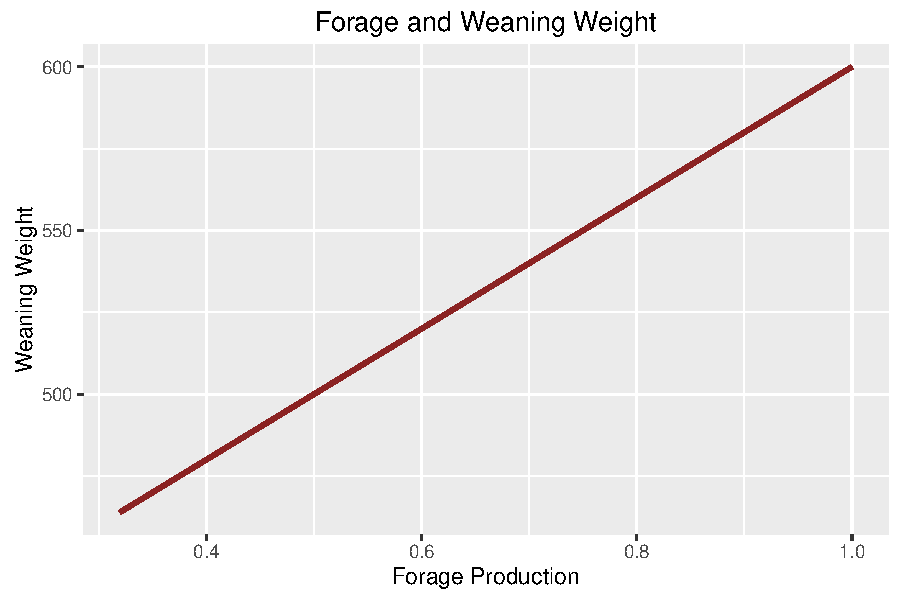
\includegraphics[width=5in]{weaningweight}



\subsection{getStationGauge}
The model is currently set for a default to the Central Plans Experimental Range (CPER), but alternative locations for COOP sites in Colorado may also be used.

\begin{itemize}
\item Function: \verb!getStationGauge!
	\begin{itemize}
	\item Description: Returns precipitation record and locational attributes for the target
  location. Default is Central Plains Experimental Range (CPER).
  \item Inputs: \verb!target.loc! (target location. default set to \verb!CPER!)
  \item Outputs: a list called \verb!station.gauge! that contains \verb!monthlyPrecipWeights! (the weight given to precipitation in each month in terms of how much it contributes to annual forage), \verb!precip! (station or gauge precipitation data from 1948 to 2015), \verb!gridCell! (Target Grid Cell for reading in PRF index values at a given point in time).
	\end{itemize}
\end{itemize}

\textbf{If CPER (default):}
\begin{enumerate}
\item Monthly precipitation weights are based on the plant growth curves for rangeland with loamy soils in major land resource area 67B (see Figure \ref{MLRA}, an area that encompasses a large portion of Eastern Colorado including the CPER site (Site ID: R067BY002CO). We use the plant growth curve for Western Wheatgrass, Blue Grama, Green Needlegrass, Fourwing Saltbush Plant Community (Growth curve number CO6701), which is well suited for grazing and is maintained with properly stocked prescribed grazing. 

\begin{figure}
\begin{center}
\label{MLRA}
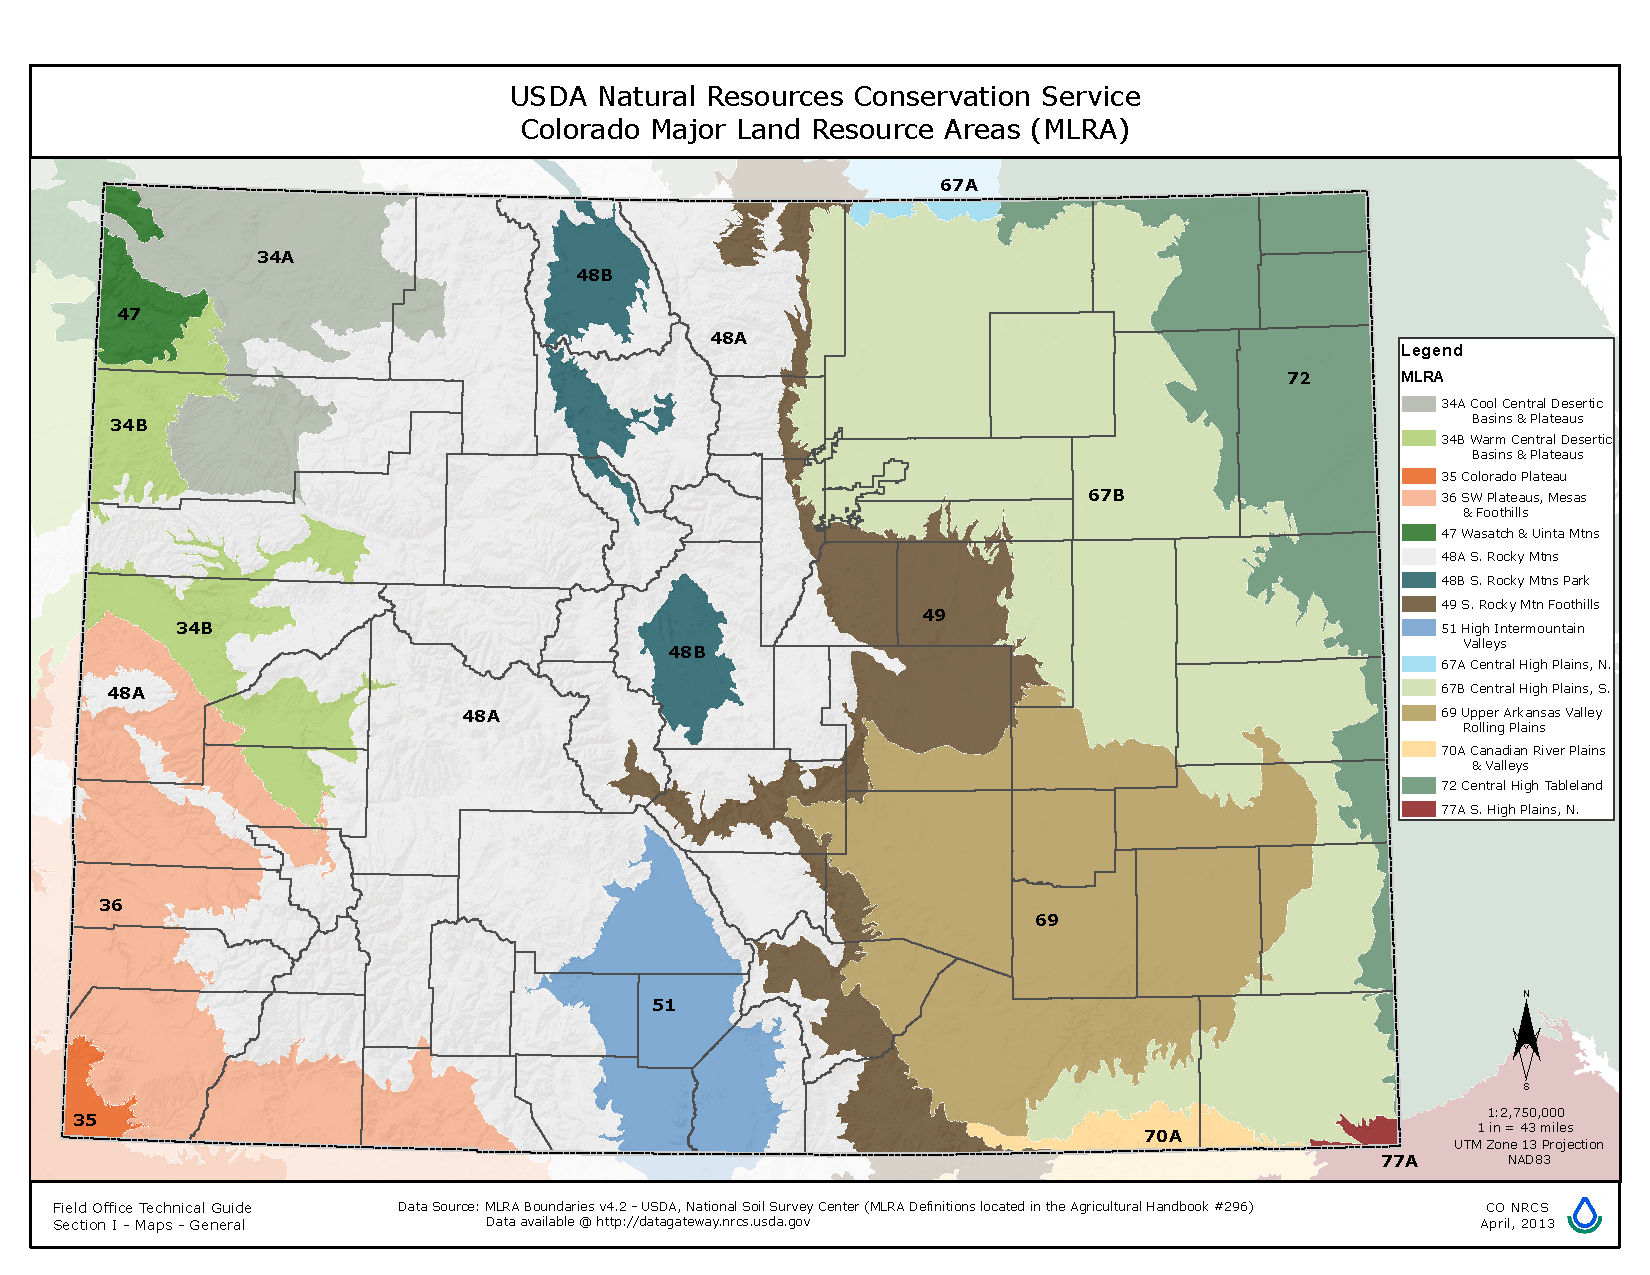
\includegraphics[scale=.5]{CO_MLRAs}
\end{center}
\caption{Major Land Resource Areas for Colorado}
\end{figure}

These monthly weights are the percentage of plant growth that is expected in each month during a normal year. Under normal conditions, total annual production averages 1300 pounds per acre. These weights add up to 1. 

\begin{tabular}{|cccccccccccc|}
\hline
Jan & Feb & Mar & Apr &May & Jun & Jul & Aug &Sep & Oct& Nov& Dec \\
\hline
0  & 0 &0.02& 0.08 &0.2 &0.28 &0.15 &0.12 &0.1 &0.05 &  0 &  0 \\
\hline
\end{tabular}

\item Station Gauge, historical precipitation totals dating back to 1948, which are also read in from the Excel model. Precip totals are collected at CPER itself and do not rely on precip data from COOP sites.
\item The target grid cell 25002 is assigned to the PRF grid cell (assuming this is the correct grid cell)
\end{enumerate}


\section{Default Model Values}

\begin{itemize}
\item Starting herd size: 600 cows
\item Ranch size: 3000 acres
\item Carrying capacity: 5 acres/cow
\item Maximum calf weaning weight: 600 lbs
\item Default calf sale rate: 75\%
\item Maximum weaning percentage: 88\%
\item Cow price: \$850/cow
\item Calf price at weaning: \$1.40/pound
\item Cow mortality rate: 4\%
\item Practice round years: 1951-1955
\item Game round years: 1999-2008
\item Household expenses: \$60,000
\item Starting cash assets: \$90,000
\item Operating costs: \$500/cow
\item Insurance Coverage Level: 90\%
\item Interest rate: 5\%
\end{itemize}



  


 \end{document}